% <!-- image -->

\begin{center}
\begin{tabular}{ll}
\toprule
Request & Response \\
\midrule
// 33042 BPP & 7 s\#x42 = RPC Response \\
\bottomrule
\end{tabular}
\end{center}

% <!-- image -->

如果 Candidate 获得了多数派的选票，说明该 Candidate 在整个集群中拥有最新的日志（比多数派成员更加完整），或者和多数派成员的日志一样完整。该 Candidate 收到的选票来自集群中拥有最完整日志的任意一个成员。

\subsubsection{领导者选举}

请求投票 RPC 的请求与响应结构体：

\begin{verbatim}
type RequestVoteRequest struct {
    term         int  // 候选人的任期号
    candidateId  int  // 请求选票的候选人的 ID
    lastLogIndex int  // 候选人的最后日志条目的索引
    lastLogTerm  int  // 候选人的最后日志条目的任期
}
\end{verbatim}

\begin{verbatim}
type RequestVoteResponse struct {
    term        int   // 当前任期号
    voteGranted bool  // 如果候选人获得选票则为真
}
\end{verbatim}

Cand 收到某个成员的消息：
\begin{itemize}
\item 若该成员的任期号大于自己的任期号，说明该成员已经晋升为 Leader，则 Candidate 变为 Follower；
\item 若该成员的任期号小于自己的任期号，可能是迟到的前任 Leader 的心跳，则忽略并继续 Leader 选举流程。
\end{itemize}

领导者选举：一个稳定的 Leader 一旦选出，就不希望进行非必要的 Leader 变更。Raft 给出了以下不等式，只要系统满足，就能选举并维护一个稳定的 Leader：

\[
\text{broadcastTime} \ll \text{electionTimeout} \ll \text{MTBF} \quad (\text{MTBF, Mean Time Between Failure})
\]

\subsection{主要内容}

\begin{enumerate}
\item 基本概念
   \begin{itemize}
   \item Term 任期
   \item 三状态机及其转换
   \item 复制状态机
   \item RPC 通信
   \end{itemize}
\item 领导者选举
\item 日志复制
\item 性能分析与优化
\item Raft 优化
\end{enumerate}

\subsubsection{日志复制}

Leader 被选出来后，怎么知道新 leader 是哪个？若正好为 leader，就可以直接开始为客户端请求提供服务，执行指令即可。

若为 follower，通过心跳告知 leader。当节点宕机，client 尝试另一个节点；接收到客户端请求的节点若知道 leader 的 ID，会将请求转发给 leader。Leader 将指令作为新的日志条目，附加到本地日志，然后复制到 followers。当该条目被超过半数 follower 复制后，leader 可以提交该条目，并应用到自己的状态机，最后把结果返回客户端。

日志结构：每条日志包含指令、任期号和日志索引号（单调递增）。一个日志索引号和任期号唯一确定一条日志。

% 图示: 日志复制过程示意
\begin{center}
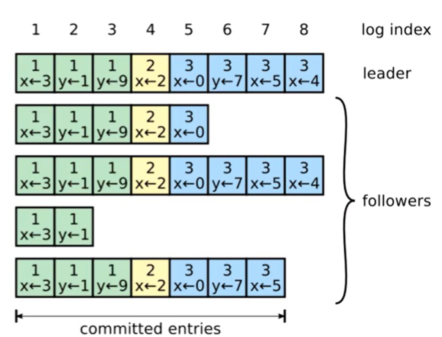
\includegraphics[width=0.8\textwidth]{figures/ch10/ch10_log_replication.png}
\end{center}

怎么让 follower 追上 leader，且所有节点的日志都完整且顺序一致？三种引起不一致的情况：
\begin{itemize}
\item follower 缓慢
\item follower 宕机
\item leader 宕机
\end{itemize}

Raft 通过一致性检查来处理：
\begin{itemize}
\item 若 follower 的日志中找不到 \texttt{prevLogIndex} 对应的条目，则拒绝此次 \texttt{AppendEntries RPC}；
\item Leader 收到拒绝后，逐步减小 \texttt{nextIndex}，重新发送，直到找到第一个二者一致的日志位置，然后复制该位置之后的所有条目；
\item Follower 中与 leader 冲突的日志条目会被 leader 的日志覆盖。因尚未提交，不违背一致性。
\end{itemize}

\textbf{一致性检查与冲突处理示例}

% 图示: 一致性检查与冲突处理
\begin{center}
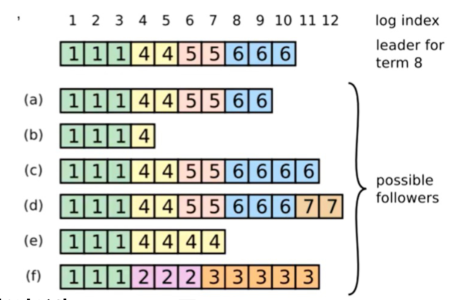
\includegraphics[width=0.8\textwidth]{figures/ch10/ch10_consistency_check.png}
\end{center}

右图最上面是当前 leader，此时 follower 中的 c 和 d 虽然比 leader 多出两个日志条目，但因为这些日志没有提交，所以不会产生冲突；leader 依靠自己的日志和选票当选（f 也可能投票给它）。多出的日志在冲突处理时会被覆盖。节点 f 拥有任期 2、3 的日志，大概说明它在那个任期内担任过 leader，但日志没有正常复制到大多数节点，也未提交。

若 leader 宕机，a、c、d 有机会成为新 leader。如果 c 或 d 当选，就可以将自己多出的日志复制给其他节点，从而使那些日志得到提交。老 leader 从宕机恢复后会成为 follower，其未提交的日志与新 leader 的日志发生冲突，通过一致性检查逐步回退，覆盖冲突内容。

追加日志 RPC 的请求与响应结构体：

\begin{verbatim}
type AppendEntriesRequest struct {
    term         int     // leader 的当前任期号
    leaderId     int     // leader 的 ID
    prevLogIndex int     // 新日志条目之前条目的索引
    prevLogTerm  int     // prevLogIndex 对应条目的任期
    entries      []byte  // 日志条目数据（为空时是心跳）
    leaderCommit int     // leader 已提交的最高日志索引
}
\end{verbatim}

\begin{verbatim}
type AppendEntriesResponse struct {
    term    int   // follower 的当前任期号
    success bool  // 若 follower 包含匹配 prevLogIndex 和 prevLogTerm 的条目则返回 true
}
\end{verbatim}

\begin{itemize}
\item \texttt{leaderCommit}：leader 确认日志被复制到大多数节点后才会提交 (Commit)，应用到自己的状态机，并通过 \texttt{leaderCommit} 字段将提交信息告知 followers。
\item Follower 收到提交信息后，会将自己已复制但未提交的日志标记为已提交，并应用到自己的状态机。
\item \texttt{response success}：只有 request 的 \texttt{term} 大于等于自己的 \texttt{term}，且通过一致性检查时，才返回 \texttt{true}；否则返回 \texttt{false}。
\end{itemize}

\textbf{日志复制：Summary}

\begin{itemize}
\item 一致性检查机制：leader 当选后无需特殊操作即可使日志恢复到一致状态，只需进行正常的 \texttt{AppendEntries} 操作；leader 从不会覆盖或删除自己的日志条目 (Append-Only)。
\item 只要过半数服务器能正常运行，Raft 就能接受并应用新日志条目，正常选出 leader 并提交日志。
\item 正常情况，新日志条目可在一次 RPC 来回中被复制到过半数机器；单个运行慢的 follower 不会影响整体性能。
\end{itemize}

\subsubsection{性能分析与优化}

基本任务：基于共识完成系统，通过 AppendEntries RPC 复制日志。理想情况下一次 RPC 即可。优化方法：
\begin{itemize}
\item \textbf{Batch（批量）}：一次网络开销可包含多个日志条目。
\item \textbf{Pipeline（流水线）}：leader 复制日志时不必等待 follower 回复，可连续发送后续 RPC。
\item 合理设置选举超时时间，平衡批量提交与延迟。
\item \textbf{Multi-Raft}：当数据量很大时，单个 Raft 的同步会成为瓶颈。可将数据划分为多个组，每组独立组成 Raft 集群，分别进行复制。但实现具有复杂性，例如如何做到负载均衡。
\end{itemize}

\subsubsection{Raft 优化}

% 原有空列表1-4，此处忽略，直接列出优点
\begin{itemize}
\item Raft 使用随机计时器进行 leader 选举，能够简单快速地实现。
\item Raft 保证首先选举出的 leader 必须拥有完整日志。
\item Raft 采用顺序日志复制的方法来避免日志空洞（非连续空洞）。
\item Raft 保证时刻都有具备完整日志的节点，可以成为 leader。
\end{itemize}

[疑似: \textbf{简单性/Simplicity}] 是 Raft 得以广泛认可与应用的关键。

% <!-- image -->

\subsection{End of Raft}
